\subsection{Gleichstrommaschine}
	Die Gleichstrommascheine besteht im Stator entweder aus Permanetmagneten, oder aus permanent-erregten Erregerwicklung. Der Rotor besteht aus Wicklungen, welche durch einen Kommutator (auch Stromwender genannt) und Bürsten mithilfe von Gleichspannung versorgt werden. Die Drehzahl der Maschine kann hierbei ganz einfach durch Verändern der Versorgungsspannung linear geregelt werden. 
	
	\begin{figure}[H]
			\centering
			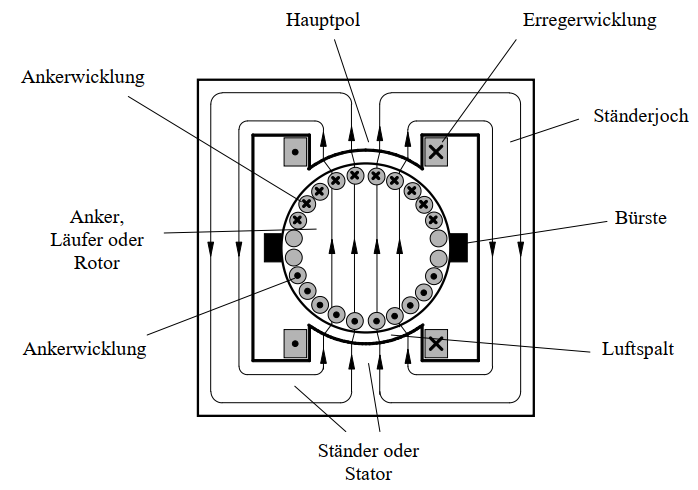
\includegraphics[scale=0.8]{./3_Stand_der_Technik/Abbildungen/Gleichstrommaschine_1}
			\caption{Aufbau Gleichstrommaschine\cite{Pischtschan2024}}
	\end{figure}
	
	Vorteil des Gleichstrommotors ist seine einfach Drehzahlregelung durch Veränderung der Spannung, Nachteil der hohe Wartungsaufwand und Verschleiß der Maschine. Er wird aufgrund von sinkenden Preisen bei Frequenzumrichtern immer weniger verwendet.